\chapter{Feature Engineering and metrics}\label{final}

The feature engineering concepts used in the experiments i.e preprocessing, postprocessing and oversampling and the metrics considered for the model evaluation are discussed here.Each section is related to each of the two experiments conducted.
Each concept used in the respective type of experiment is explained in each sub section of the sections.

\section{Anomaly detection}
Extensive exploratory data analysis and preprocessing was performed on the datasets before developing the Isolation forest model. The concepts used for anomaly detection were:

\subsection{t-SNE(t-distributed stochastic neighbor embedding)}
t-SNE is used to visualize high dimensional data. The similarities between the data points are converted to joint probabilities and the Kullback-Leibler divergence between these joint probabilities of the low-dimensional embedding and the high-dimensional data is minimized. The similarities between the pairs of instances in the high dimensional space and low dimensional space are optimized using a cost function.

\section{Deep leaning regression}
Deep learning models are built to predict the number of faults corresponding to a datapoint in the testing dataset. Since the predictions are strictly greater than zero we have used ReLU Activation function after the output layer in the models and post processing is performed after that to convert the predictions to whole numbers. Different concepts used in the feature engineering in these experiments are:

\subsection{Min Max Scaling}
Min Max scaling is done to rescale a feature or observation value to a distribution value between 0 and 1. The formula followed is:
 \begin{figure}
\makebox[\textwidth][c]{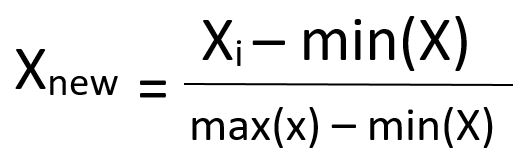
\includegraphics[width=0.2\textwidth]{others/minmaxscaling.jpg}}%
  \caption{Min Max scaling formula}
  \label{fig:key}
\end{figure}

\subsection{SVD(Singular Value Decomposition)}
The singular value decomposition (SVD) is a factorization of a real or complex matrix that generalizes the eigendecomposition of a square normal matrix to any. matrix via an extension of the polar decomposition.

\subsection{PCA(Principal Component Analysis)}
Principal Component Analysis, or PCA, is a dimensionality-reduction method that is often used to reduce the dimensionality of large data sets, by transforming a large set of variables into a smaller one that still contains most of the information in the large set.
Reducing the number of variables of a data set naturally comes at the expense of accuracy, but the trick in dimensionality reduction is to trade a little accuracy for simplicity. 


\subsection{Over Sampling}
Oversampling  in data analysis are techniques used to adjust the class distribution of a data set.
The bias in the training dataset can influence many machine learning algorithms, leading some to ignore the minority class entirely.To address this problem ,oversampling is carried out on the dataset .Random Oversampling involves supplementing the training data with multiple copies of some of the minority classes. Oversampling can be done more than once.
\subsubsection{Synthetic Minority Over-sampling Technique(SMOT)}
The most common technique to oversample a dataset used in a typical classification problem is SMOTE: Synthetic Minority Over-sampling Technique.To illustrate how this technique works consider some training data which has s samples, and f features in the feature space of the data. Note that these features, for simplicity, are continuous. As an example, consider a dataset of birds for classification. The feature space for the minority class for which we want to oversample could be beak length, wingspan, and weight (all continuous). To then oversample, take a sample from the dataset, and consider its k nearest neighbors (in feature space). To create a synthetic data point, take the vector between one of those k neighbors, and the current data point. Multiply this vector by a random number x which lies between 0, and 1. Add this to the current data point to create the new, synthetic data point.\cite{smot}

\subsection{FPA(Fault-percentile-average)}
Considering m modules f1 , f2 , . . . ,fm listed in increasing order of predicted defect number, si as the actual defect number in the module fi, and s = s1 + s2 + ... + sm as the total number
of defects in all the modules, the proportion of actual defects in the top t predicted modules (i.e., top t modules predicted to have most defects) to the whole defects is \(\frac{1}{s}\sum_{i=m-t+1}^{m}s_i\). Then FPA is defined as follows:
\[\frac{1}{m}\sum_{t=1}^{m} \frac{1}{s}\sum_{i=m-t+1}^{m}s_i\] 

\subsection{CLC(Cumulative lift chart (also the area under CLC))}

CLC uses percentages of modules as x-axis and percentages of defects as y-axis. The area under CLC is always used for comparison, and the area is simply denoted as CLC in this paper.Considering m modules f1 , f2 , ..., fm , listed in increasing order of predicted defect number, si as the actual defect number in the module fi, and s = s1 + s2 + ... + sm as the total number of defects in all the modules, the area under the curve should be computed as the sum of areas of trapezoid composed of two adjacent points and the axes in the CLC. Using CLC to denote
the area under the curve in rest of the paper, it can be computed as follows:\cite{clc}
\[CLC = \sum_{t=1}^{m}trapezoid_t\]
\[=(\frac{1}{m})(\frac{1}{2})((0+\frac{s_m}{s}+...\]
\[+(\frac{s_m+...+s_2}{s}+\frac{s_m+....+s_1}{s}))\]

